Til de følgende opgaver udvider vi typen \texttt{figure} med en mulighed for at repræsentere trekanter:

\begin{lstlisting}[numbers=none,frame=none,mathescape]
type figure =
  | Circle of point * int * colour
     // defined by center, radius, and colour
  | Rectangle of point * point * colour
     // defined by corners bottom-left, top-right, and colour
  | Mix of figure * figure
     // combine figures with mixed colour at overlap
  | Triangle of point * point * point * colour
     // defined by the three points and colour
\end{lstlisting}

\noindent
Konstruktøren \texttt{Triangle} tager tre punkter og en farve som
argument. Der er intet krav til hvordan de tre punkter er placeret i
forhold til hinanden.

For at bestemme hvorvidt et punkt er placeret inde i en trekant
benytter vi os af et trick der forudsætter at vi kan beregne arealet
af en trekant ved at kende dens hjørnepunkter. Det viser sig at hvis
en trekant er bestemt af punkterne $p_1=(x_1,y_1)$, $p_2=(x_2,y_2)$ og
$p_3=(x_3,y_3)$ vil følgende relativt simple formel kunne benyttes til
at udregne arealet:
\[
\emph{area} = \left | \dfrac{x_1(y_2-y_3) + x_2(y_3-y_1) + x_3(y_1-y_2)}{2} \right |
\]

\begin{minipage}{.62\textwidth}

  Tricket som vi nu skal benytte til at afgøre om et punkt $p$ ligger
  inden i en trekant udspændt af hjørnerne $p_1$, $p_2$ og $p_3$
  forklares lettest ved at iagttage figuren til højre. Såfremt arealet
  af de tre trekanter $(p_1, p_2, p)$, $(p_2,p_3,p)$, og $(p_1,p_3,p)$
  tilsammen er større end arealet af trekanten $(p_1,p_2,p_3)$, da
  ligger punktet $p$ udenfor trekanten $(p_1,p_2,p_3)$; ellers ligger
  punktet indenfor trekanten.

\end{minipage} \hfill \begin{minipage}{.35\textwidth}
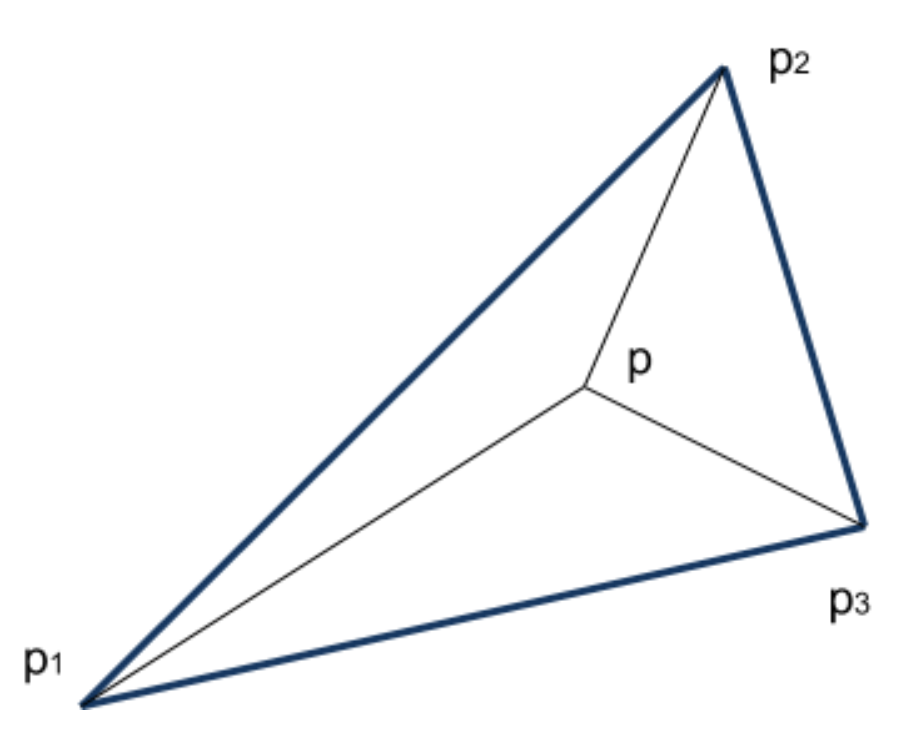
\includegraphics[width=0.9\textwidth]{triarea.png}
\end{minipage}
